% Když budete cokoli psát: ukládejte starší verze vždy odděleně, abyste se 
% k nim mohli kdykoli vrátit. Kusy textu, které jste se rozhodli nepoužít, taky ukládejte do zvláštního souboru. Smazat se to dá vždycky, ale psát to znova je opruz. 

% A POŘÁD ZÁLOHUJTE. POŘÁD !!!

\documentclass[12pt, a4paper, oneside]{article} 
% velikost písma, stránky, typ dokumentu -- detaily viz literatura

\usepackage{czech} % nastavení češtiny
%\usepackage[latin2]{inputenc}
%\usepackage[cp1250]{inputenc} % pro win1250
\usepackage[center]{caption} 
\usepackage[utf8]{inputenc}
\usepackage{wrapfig} % nastavení obtékání textu
\usepackage{graphicx,amsmath} % nastavení grafiky, matematiky
\usepackage{subfig} % více obrázků vedle sebe 
\usepackage{float}
\usepackage{amsmath}
\usepackage{amssymb}
\usepackage{bbding}
\usepackage{enumitem}
\usepackage{breakurl}
%\usepackage{indentfirst}

\usepackage{tocloft} %přidá tečky do obsahu ke kapitolám /sekcím 
\renewcommand{\cftsecdotsep}{\cftdotsep}

\usepackage[bookmarksopen,colorlinks,plainpages=false,linkcolor=black,urlcolor=blue,citecolor=black,filecolor=black,menucolor=black,unicode=true]{hyperref}

\urlstyle{rm}
%bookmarksopen -- open up bookmark tree 
%colorlinks -- zbarví odkazy (implicitně orámovaný nezbarvený text)
%urlcolor -- barva odkazů (implicitně magenta) 
%linkcolor=black -- barva odkazů v obsahu (implicitně red)


\usepackage{listings}
\usepackage{color}
\definecolor{lightgray}{rgb}{.9,.9,.9}
\definecolor{darkgray}{rgb}{.4,.4,.4}
\definecolor{purple}{rgb}{0.65, 0.12, 0.82}

\lstdefinelanguage{JavaScript}{
  keywords={typeof, new, true, false, catch, function, return, null, catch, switch, var, if, in, while, do, else, case, break, for},
  keywordstyle=\color{blue}\bfseries,
  ndkeywords={class, export, boolean, throw, implements, import, this},
  ndkeywordstyle=\color{darkgray}\bfseries,
  identifierstyle=\color{black},
  sensitive=false,
  comment=[l]{//},
  morecomment=[s]{/*}{*/},
  commentstyle=\color{purple}\ttfamily,
  stringstyle=\color{red}\ttfamily,
  morestring=[b]',
  morestring=[b]"
}

\lstset{
   language=JavaScript,
   backgroundcolor=\color{lightgray},
   extendedchars=true,
   basicstyle=\footnotesize\ttfamily,
   showstringspaces=false,
   showspaces=false,
   numbers=left,
   numberstyle=\footnotesize,
   numbersep=9pt,
   tabsize=2,
   breaklines=true,
   showtabs=false,
   aboveskip=5mm,
   belowskip=7mm,
   captionpos=b
}

\renewcommand{\lstlistingname}{Příklad}

% \usepackage{parskip} -- zapne americké odstavce v celé práci

\addtolength{\textwidth}{-2mm} 
\addtolength{\hoffset}{4mm}  % posun textu kvůli kroužkové vazbě  

\setlength{\intextsep}{5mm} % nastavení mezery okolo obrázků

% nastavení příkazu >\figcaption pro popis čehokoli, jako by to byly obrázky 
\makeatletter   
\newcommand\figcaption{\def\@captype{figure}\caption}
\makeatother

\renewcommand\refname{Literatura} 
%\def\bibname{PŘÍLOHA D: Reference}
%\renewcommand\bibname{PŘÍLOHA D: Reference}
% přejmenuje anglický název Reference na české Literatura


%\makeindex % příprava pro výrobu indexu (jestli ho chcete)

%%    VLNKA <fileinput>  KkSsVvZzOoUuAaIi        
% Defaultni  koncovka pro <fileinput> je  ".tex"
%FIXME: haze error
%\cstieon % Vypne chovani vlnky jako tvrde mezery v matematickem rezimu

%%%%%%%%%%%%%%%%%%%%%%%%%%%%%%%%%%%%%%%%%%%%%%%%%%%%%%%%%%%%%%%
%V PROSTŘEDÍ ROVNIC SE NESMÍ VYSKYTOVAT PRÁZDNÝ ŘÁDEK
%
%PROGRAMY VLNKA A CSINDEX SE MUSÍ SPUSTIT SAMOSTATNĚ
%%%%%%%%%%%%%%%%%%%%%%%%%%%%%%%%%%%%%%%%%%%%%%%%%%%%%%%%%%%%%%%

% definice příkazů 
\newcommand{\D}{\medskip \noindent} % nový odstavec v "americkém" formátování 
\newcommand{\B}{\textbf} %tučné písmo
\newcommand{\A}{\mathbf} %tučné písmo v matematickém režimu
\newcommand{\TO}{\ensuremath{\boldsymbol\Omega}} % tučný znak velké omega -- pro ohmy
\newcommand{\I}{\index}  % vytváří položku indexu (asi nepoužijete)
\newcommand{\Deg}[1][]{\ensuremath{{#1}^\circ}} % vysází značku stupně Celsia
\newcommand{\Def}{\footnotesize Definice: \normalsize}
\newcommand{\Pos}{\footnotesize Experiment: \normalsize}
\newcommand{\Odv}{\footnotesize Odvození: \normalsize}
\newcommand{\Vym}{\footnotesize Vymezení pojmu: \normalsize}
\newcommand{\Ob}{obrázek }
\newcommand{\It}{\textit}  % kurzíva
\newcommand{\M}{\mathrm}   % v prostředí rovnic nastaví normální písmo (místo kurzívy ) 
\newcommand{\F}{\footnotesize} % zmenšená velikost písma
\newcommand{\N}{\normalsize} % normální velikost písma
%\newcommand{\U}{\underline}  % podtržené písmo
\newcommand{\e}{\ensuremath} 
\newcommand{\Has}{\textcolor{green}{\CheckmarkBold}}
\newcommand{\NoHas}{\textcolor{red}{\XSolidBrush}}
% další příkaz se aplikuje, pouze, když jste v matematickém režimu

%\hyphenation{Pusť-me pla-tí hod-no-ty do-sa-dí-me za-da-né dal-ším}
% dělení slov, kdyby implicitní nevyhovovalo

\linespread{1.3} 
% řádkování 1,5x  
% použijete podle situace  

\unitlength=1mm % nastavení volby jednotek 

% konec hlavičky
%%%%%%%%%%%%%%%%%%%%%%%%%%%%%%%%%%%%%%%%%%%%%%%%%%%%%%%%%%%%%%%%%%%
%%%%%%%%%%%%%%%%%%%%%%%%%%%%%%%%%%%%%%%%%%%%%%%%%%%%%%%%%%%%%%%%%%%

\begin{document} % začátek textové části 

% titulní strana
\pagestyle{empty} % vynechá číslování
 
\voffset = -20mm % posun začátku textu výš
\enlargethispage{60mm} % zvětší oblast tisku pro tuto stránku   

\begin{center}
 
\Large \B{STŘEDOŠKOLSKÁ ODBORNÁ ČINNOST}

\vspace{60mm}

\huge %\LARGE
\B{LORRIS TOOLBOX \\ Sada nástrojů pro vývoj a~řízení robotů}
% na titulní straně může být stručnější, pokud je to potřeba  

\Large

\vspace{90mm}


\B{Vojtěch Boček} \\

\vspace{40mm}

\B{Brno 2012}


\end{center}

\newpage % konec titulní strany 
%%%%%%%%%%%%%%%%%%%%%%%%%%%%%%%%%%%%%%%%%%%%%%%%%%%%%%%%%%%%%%%%%%%%%%%%%%%

% vnitřní titulní strana
\voffset = -20mm % posun začátku textu výš
\enlargethispage{60mm} % zvětší oblast tisku pro tuto stránku   

\begin{center}

\Large \B{STŘEDOŠKOLSKÁ ODBORNÁ ČINNOST}  \\
\vspace{10mm}
 \normalsize 
\B{Obor SOČ: 18. Informatika}% číslo a název -- vyplníme spolu 

\vspace{45mm}

\LARGE %\huge 
\B{LORRIS TOOLBOX \\ Sada nástrojů pro vývoj a~řízení robotů}%SADA NÁSTORUJŮ PRO VÝVOJ A ŘÍZENÍ ROBOTŮ} 
\end{center}  
\large

\vspace{50mm}


\begin{tabbing}
\hspace{10mm} \= \hspace{30mm}  \=   \kill % nastavení zarážek 
  \> \B{Autor:}  \> \B{Vojtěch Boček}        \\[8mm] 
  \> \B{Škola:}   \> \B{SPŠ a~VOŠ technická, }     \\
  \>              \> \B{Sokolská 1 602 00 Brno}    \\[8mm]

  \> \B{Konzultant:} \> \B {Jakub Streit} 
\end{tabbing}

\vspace{20mm}

\begin{center}
\B{Brno 2012}

\end{center}
\normalsize
%%%%%%%%%%%%%%%%%%%%%%%%%%%%%%%%%%%%%%%%%%%%%%%%%%%%%%%%%%%%%%%%%%%%%%%%%%%
\newpage  % Prohlášení o autorství  
\voffset = 0mm % posun začátku textu zpět

~ % musí to tu být, aby fungovala svislá mezera

\vspace{10mm}

\section*{Prohlášení}

Prohlašuji, že jsem svou práci vypracoval samostatně, použil jsem pouze 
podklady (literaturu, SW atd.) citované v~práci a~uvedené v~přiloženém seznamu 
a~postup při zpracování práce je v~souladu se zákonem č. 121/2000 Sb., o~právu 
autorském, o~právech souvisejících s~právem autorským a~o~změně některých 
zákonů (autorský zákon) v~platném znění. 
 
\vspace{20mm} 
 
\noindent V~Brně  dne: 6.3.2012 \hspace{50mm}                 podpis:   
 

%%%%%%%%%%%%%%%%%%%%%%%%%%%%%%%%%%%%%%%%%%%%%%%%%%%%%%%%%%%%%%%%%%%%%%%%%%%
\newpage   % Poděkování -- nepovinné 

~ % musí to tu být, aby fungovala svislá mezera

\vspace{120mm}

\section*{Poděkování}
Děkují Jakubu Streitovi za rady, obětavou pomoc, velkou trpělivost a~podnětné připomínky poskytované během práce na tomto projektu, Martinu Vejnárovi za informace o programátoru Shupito, panu profesorovi Mgr. Miroslavu Burdovi za velkou pomoc s prací a v neposlední řadě Martinu Foučkovi za rady a pomoc při práci s Qt Frameworkem. Dále děkuji organizaci DDM Junior za poskytnutí podpory.

\D Tato práce byla vypracována za finanční podpory JMK.
 

%%%%%%%%%%%%%%%%%%%%%%%%%%%%%%%%%%%%%%%%%%%%%%%%%%%%%%%%%%%%%%%%%%%%%%%%%%%
\newpage   % Anotace 
~ % musí to tu být, aby fungovala svislá mezera
\vspace{10mm}

\section*{Anotace }


Tato práce popisuje sadu nástrojů pro vývoj a ovládání libovolného zařízení schopného komunikovat po sériové lince nebo TCP socketu.

Aplikace zastřešuje několik modulů. Každý modul je určen pro specifickou činnost -- parsování a zobrazování dat, programování mikročipů atd.

Hlavním přínosem tohoto softwaru je, že výrazně urychluje, zpřehledňuje a zjednodušuje vývoj a testování aplikací pro mikročipy, typicky programování a řízení různých druhů robotů.
%Hlavní oblastí použití jsou čtení, parsování a zobrazování dat z mikročipů, 

    %Cílem této práce bylo vytvořit uživatelské prostředí určené k parsování a~zobrazování surových dat posílaných z mikrokontrolérů v~robotech, digitálních sondách apod. 
%Hlavní vlastností programu je modulárnost -- rozdělení na~podčásti určené ke specifickým úkonům (Terminál, grafický parser, vykreslování grafů).

\D \B{Klíčová slova:} analýza dat, počítačový program, robot, grafické zobrazení, vývoj a testování aplikací

\section*{Annotation}

This labor describes toolbox designed for developement and control of any device capable of connecting to serial port or TCP socket.

This application contains several modules. Each module is designed for one particular function -- parsing and displaying data, programming microcontrollers etc.

Main asset of this software is quick, well arranged and simple developement and testing of applications for microcontrollers -- typically programming and controling various kinds of robots.

    %Purpose of this labor is to create graphical user interface for parsing and displaying raw data sent from embedded devices, robots, digital probes and other devices which are using microcontrollers.
%Main feature of this application is modularity -- it is divided to sub-sections designed for specific operations (Terminal, graphical parser, graph drawer).

\D \B{Key words:} data analysis, computer program, robot, graphical interface, developement and testing of applications

\addtolength{\textheight}{30mm} % prodlouží následující stránku

%%%%%%%%%%%%%%%%%%%%%%%%%%%%%%%%%%%%%%%%%%%%%%%%%%%%%%%%%%%%%%%%%%%%%%%%%%%
\newpage
\pagestyle{plain}

\setlength{\voffset}{-20mm} % posune text/obrázek na této stránce nahoru
\setcounter{page}{1}  % nastaví čítač stránek znovu od jedné

\tableofcontents  % vysází obsah

\addtolength{\textheight}{-30mm} % zkrátí následující stránku
%%%%%%%%%%%%%%%%%%%%%%%%%%%%%%%%%%%%%%%%%%%%%%%%%%%%%%%%%%%%%%%%%%%%%%%%%%%
\newpage
\setlength{\voffset}{0mm} % posune text/obrázek na této stránce, kam patří
%\pagestyle{headings} % znovu zapne číslování
\pagestyle{plain}
\section*{Úvod}

\addcontentsline{toc}{section}{Úvod} % přidá položku úvod do obsahu
% zde začne text úvodu
Při stavbě robotů na robotické soutěže jsem se setkal s problémem zpracovávání dat z poměrně velkého množství senzorů (několik ultrazvukových měřáků vzdálenosti, enkodéry, které měří ujetou vzdálenost, tlačítka hlídající náraz do mantinelu, ...), které robot obsahuje, a jejich přehledného zobrazování. 
%Nenašel jsem žádný program, který by mi vyhovoval.
\subsection*{Požadavky na aplikaci}
\addcontentsline{toc}{subsection}{Požadavky na aplikaci}
Od programu vyžaduji tyto vlastnosti:
\begin{enumerate}
    \item Možnost zpracovávat data přicházející ze zařízení a přehledně je zobrazovat % 1
    \item Podpora co nejvíce formátů příchozích dat % 2
    \item Snadné a rychlé používání % 3
    \item Možnost běhu i na jiných systémech než je MS Windows % 4
    \item Co možná nejnižší cena % 5
    \item Snadná rozšířitelnost (ideálně otevřený zdrojový kód) % 6
    \item Nezávislost na další aplikaci (např. MS Office Excel) % 7
\end{enumerate}

% Z tohoto důvodu jsem se rozhodl napsat vlastní program.

\subsection*{Existující programy}
\addcontentsline{toc}{subsection}{Existující programy}
Aplikací, které mají podobné určení (tj. vyčítání dat ze sériového portu a jejich zobrazování), jsem našel pouze několik. K dispozici jsou buď komerční aplikace, které stojí poměrně velké množství peněz (a přesto nesplňují všechny požadavky), anebo aplikace, které dokáží zobrazovat data pouze v jednom formátu -- typicky graf.

\begin{itemize}
    \item {\bf SerialChart}\cite{serialchart} je open-source program\footnote{Program s otevřeným zdrojovým kódem} pro parsování a zobrazování dat přicházející ze sériového portu. Je jednoduchý a přehledný, dokáže však zobrazovat pouze graf a nastavení je třeba ručně napsat.
    \item {\bf WinWedge}\cite{winwedge} je komerční program který dokáže zpracovávat data přicházející sériovým portem a zobrazovat je jako graf v MS Excel nebo ve webové stránce. Dokáže také posílat příkazy zpět do zařízení, má však horší ovládání a užší možnosti použití (hlavně kvůli nutnosti použít další program pro zobrazování). Je dostupný pouze pro MS~Windows a základní verze stojí \$ 259.
    \item {\bf Advanced Serial Data Logger}\cite{serialdatalogger} je zaměřený primárně na export dat ze sériové linky do souboru, data dokáže zobrazovat pouze přeposláním do jiné aplikace (např. MS Office Excel), podobně jako WinWedge.
    \item {\bf StampPlot Pro}\cite{stamplot} dokáže zobrazovat příchozí data ve widgetech zvolených uživatelem, má však komplikované ovládání, nemá otevřený zdrojový kód, je dostupný pouze pro MS Windows a pod verzí 7 nefunguje.
% pod win Xp se pripoji
\end{itemize}


\subsection*{Porovnání aplikací}
\addcontentsline{toc}{subsection}{Porovnání aplikací}
Následující tabulka shrnuje funkce a vlastnosti jednotlivých programů. Číslování požadavků odpovídá seznamu v kapitole \uv{Požadavky na aplikaci}.

\vspace{5mm}

\begin{tabular}{ | l | l | l | l | l | l | l | l |}
    \hline
    Požadavky:                  & 1      & 2      & 3      & 4      & 5      & 6      & 7      \\ \hline
    SerialChart                 & \Has   & \NoHas & \Has   & \NoHas & \Has   & \Has   & \Has   \\ \hline 
    WinWedge                    & \NoHas & \Has   & \Has   & \NoHas & \NoHas & \NoHas & \NoHas \\ \hline 
    Advanced Serial Data Logger & \NoHas & \Has   & \Has   & \NoHas & \NoHas & \NoHas & \NoHas \\ \hline 
    StampPlot Pro               & \Has   & \Has   & \NoHas & \NoHas & \Has   & \NoHas & \Has   \\ \hline 
%    Lorris                      & \Has   & \Has   & \Has   & \Has   & \Has   & \Has   & \Has   \\ \hline 
\end{tabular}

\vspace{5mm}

Z těchto důvodů jsem se rozhodl napsat vlastní aplikaci, která bude všechny výše uvedené požadavky splňovat.

\section{Popis rozhraní}
%\addcontentsline{toc}{section}{Popis rozhraní}
Svůj program jsem pojmenoval \uv{Lorris}, je vytvořený v C++ a využívá Qt Framework\cite{qtfrm} (v4.7), což je multiplatformní framework, který mimo jiné umožňuje spustit aplikaci na více operačních systémech -- testoval jsem na Debian Linux\cite{debian} (Wheezy, 64bit) a Windows 7.

\subsection{Web a repozitář programu}
%\addcontentsline{toc}{subsection}{Web a repozitář programu}
GIT\footnote{\It{GIT} -- distribuovaný systém správy verzí} repozitář programu jsem vytvořil na serveru GitHub\cite{github}, který kromě hostingu repozitáře poskytuje i několik dalších služeb, mezi nimi i hosting webu projektu. Na webu, který jsem vytvořil, jsou odkazy ke stažení spustitelných souborů pro Windows, popis programu, video s představením programu (6 min.), ukázky z programu (screenshoty) a návod ke zkompilování pro MS Windows a Linux.

\begin{itemize}
    \item Repozitář: \url{https://github.com/Tasssadar/Lorris}
    \item Web (česká verze):\\ \url{http://tasssadar.github.com/Lorris/cz/index.html}
    \item Web (anglická verze):\\ \url{http://tasssadar.github.com/Lorris/index.html}
    \item Prezentace práce: \\ \burl{http://www.sokolska.cz/soc-2012/bocek-vojtech-lorris-sada-nastroju-pro-robotiku/}
\end{itemize}
V repozitáři nadále probíhá aktivní vývoj.
%Prezentace práce: \\ \url{http://www.sokolska.cz/soc-2012/bocek-vojtech-lorris-sada-nastroju-pro-robotiku/}
\subsection{Struktura aplikace}
%\addcontentsline{toc}{subsection}{Struktura aplikace}
Program je navrhnutý jako modulární aplikace, aby mohl zastřešit několik samostatných částí, které však mají podobnou oblast použití. Základní část programu poskytuje připojení k zařízení (např. robot, deska s čipem) a ukládání nastavení aplikace, samotné zpracování dat probíhá v modulech, které jsou otevírány v panelech -- podobně jako stránky ve webovém prohlížeči.\\
\\
Možnosti připojení k zařízení:
\begin{itemize}
    \item Sériový port
    \item Shupito Tunel (virtuální sériový port, viz kapitola \ref{tunel})
    \item TCP socket\footnote{\It{Transmission Control Protocol} -- připojení přes internet.}
    \item Načtení dat ze souboru
\end{itemize}
Je možné mít připojeno více různých modulů na jedno zařízení.  

\begin{figure}[H]
\begin{center}
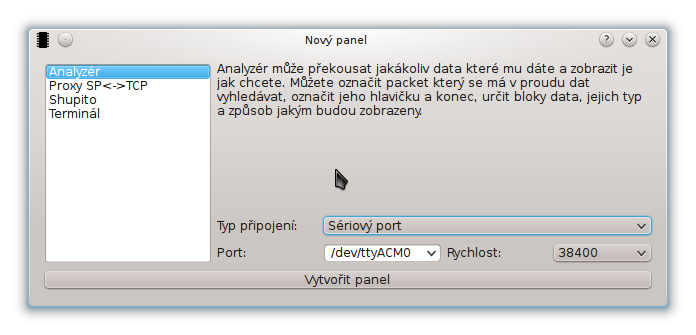
\includegraphics[width=\textwidth]{img/con_dialog.png}
\caption{Dialog vytvoření panelu}
\end{center}
\end{figure}

\newpage
\section{Modul: Analyzér}
%\addcontentsline{toc}{section}{Modul: Analyzér} 
%\addcontentsline{toc}{subsection}{Popis}

\begin{figure}[h]
\begin{center}
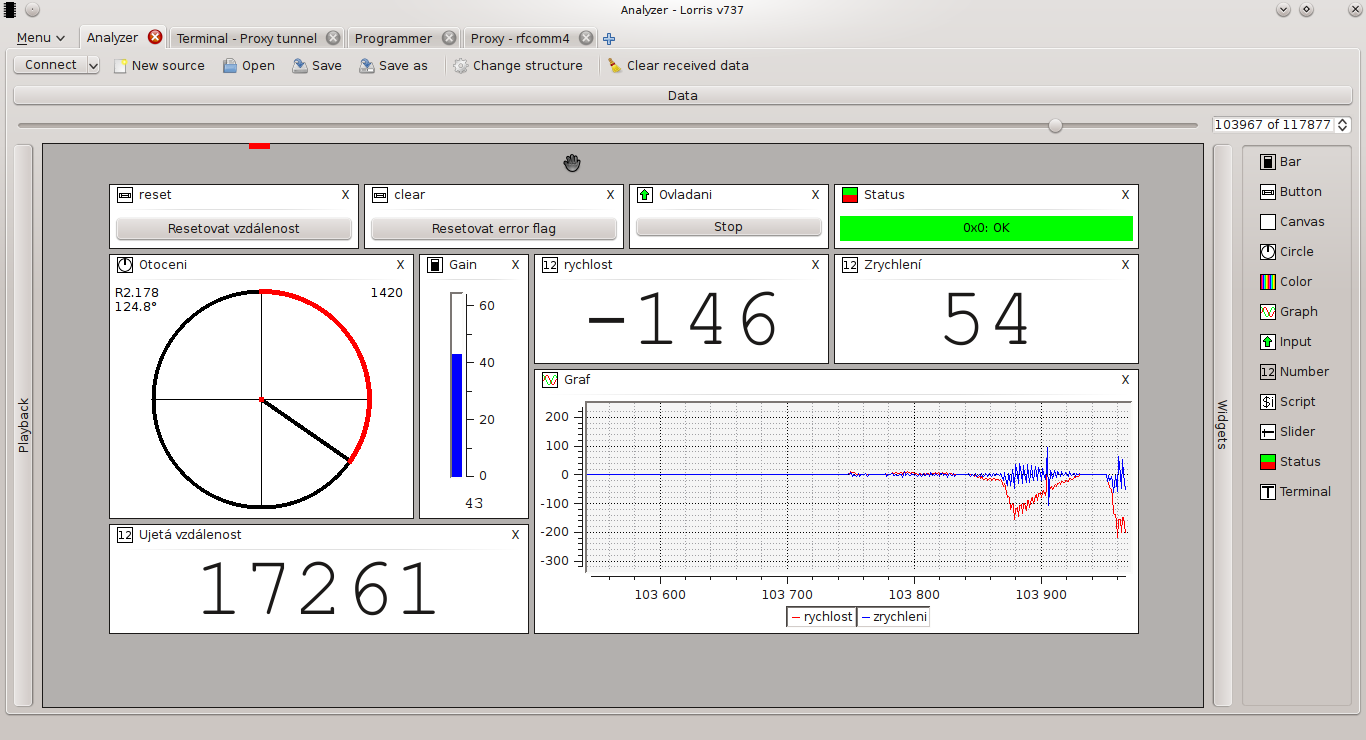
\includegraphics[width=\textwidth]{img/analyzer_all.png}
\caption{Modul analyzér}
\label{Analyzer}
\end{center}
\end{figure}

Tento modul parsuje data (strukturované do packetů) přicházející ze zařízení a zobrazuje je v grafických \uv{widgetech}. Zpracovaná data si aplikace ukládá do paměti -- listování packety je možné pomocí posuvníku a boxu v horní části okna. Data (přijatá data, struktura packetů a rozestavení a nastavení widgetů) je také možné uložit do souboru a později zase v programu otevřít.  

Struktura dat se nastavuje v samostatném dialogu (viz obrázek \ref{Analyzer_struct}), kde je možno nastavit délku packetu, jeho endianness\footnote{\It{Endianness} -- pořadí uložení bytů v paměti počítače}, přitomnost hlavičky a její obsah -- statická data (\uv{start byte}), délka packetu (pokud je proměnná), příkaz a ID zařízení. Podle příkazu a ID zařízení je možno později data filtrovat.


\newpage
\setlength{\voffset}{0mm} % posune text/obrázek na této stránce, kam patøí
\pagestyle{plain}

Po nastavení struktury se přijatá data začnou po packetech zobrazovat v horní části okna, a v pravé části se zobrazí sloupeček s dostupnými zobrazovacími widgety. Widgety se dají pomocí drag\&drop principu \uv{vytahat} na plochu v prostřední části okna. Data se k widgetu přiřadí taktéž pomocí drag\&drop, tentokrát přetažení prvního bytu dat na widget. 

Poté widget zobrazuje data tohoto bytu, nebo tento byte bere jako první, pokud jsou data delší. Aby bylo možné zpětně poznat, který byte je k widgetu přiřazen, je po najetí myši na widget červeně zvýrazněn.

Nastavení widgetu jsou přistupná v kontextovém menu po pravém kliknutí myší na widget. Nastavit lze jméno a další parametry podle typu widgetu -- podrobněji jsou možnosti nastavení popsány u jednotlivých widgetů. Widgety je taktéž možné \uv{uzamknout}, aby nebylo možné je zavřít, měnit jejich pozici a velikost.
%(jeho jméno, u čísla např. jeho datový typ apod. -- podrobněji jsou možnosti nastavení popsány  u jednotlivých widgetů)

\begin{figure}[h]
\begin{center}
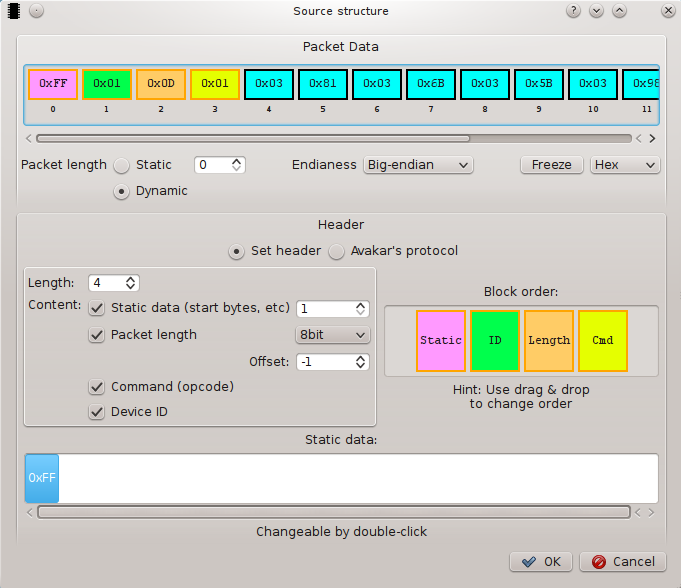
\includegraphics[scale=0.7]{img/analyzer_struct.png}
\caption{Dialog nastavení struktury dat}
\label{Analyzer_struct}
\end{center}
\end{figure}

\begin{figure}[H]
\begin{center}
\subfloat[Seznam widgetů]{\label{analyzer_widgets}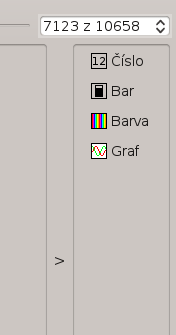
\includegraphics[scale=1]{img/analyzer_widgets.png}}
\hfill
\subfloat[Přiřazení dat pomocí drag\&drop]{\label{analyzer_widgets}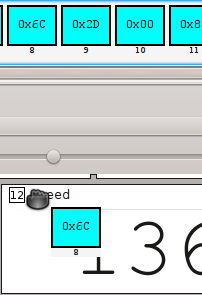
\includegraphics[scale=1]{img/analyzer_drag_data.png}}  
\caption{Widgety}
\label{widgets}
\end{center}
\end{figure}

\subsection{Widget: číslo}
%\addcontentsline{toc}{subsection}{Widget: číslo}
\begin{figure}[h]
\begin{center}
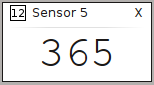
\includegraphics{img/w_num.png}
\caption{Widget: číslo}
\end{center}
\end{figure}
Tento widget dokáže zobrazovat celá čísla (se znaménkem i bez, 8 až 64 bitů dlouhé) a desetinná čisla (single-precision\footnote{Standartní formát uložení desetinných čísel v jazyku C a dalších (standart IEEE 754-2008).}, 32bit a 64bit).\\
Widget dále dokáže zarovnat číslo na maximální délku jeho datového typu\\a~formátovat ho těmito způsoby:
\begin{itemize}
    \item Desítkový -- číslo v desítkové soustavě
    \item Desítkový s exponentem -- použije exponent pro zapsaní velkých čísel. Dostupné pouze pro desetinná čísla.
    \item Hexadecimální -- výpis v šestnáctkové soustavě. Dostupné pouze pro přirozená čísla. 
    \item Binární -- zobrazí číslo ve dvojkové soustavě.  Dostupné pouze pro přirozená čísla.
\end{itemize}


%\newpage
\subsection{Widget: sloupcový bar}
%\addcontentsline{toc}{subsection}{Widget: sloupcový bar}
\begin{figure}[H]
\begin{center}
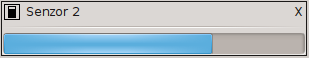
\includegraphics{img/w_bar.png}
\caption{Widget: sloupcový bar}
\end{center}
\end{figure}
Widget zobrazuje hodnotu ve sloupcovém baru. Lze nastavit datový typ vstupních dat (stejně jako u čísla), orientaci (vertikální nebo horizontální) a rozmezí zobrazovaných hodnot.

\subsection{Widget: barva}
%\addcontentsline{toc}{subsection}{Widget: barva}
\begin{figure}[H]
\begin{center}
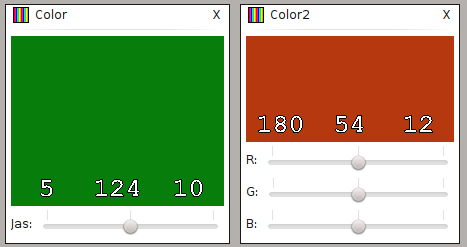
\includegraphics{img/w_col.png}
\caption{Widget: barva}
\end{center}
\end{figure}
Tento widget ukáže 24-bitové hodnoty RGB jako barevný obdélník. Dokáže provést korekci jasu všech barev nebo každé z barev RGB zvlášť.

%\newpage
\subsection{Widget: graf}
%\addcontentsline{toc}{subsection}{Widget: graf}
\begin{figure}[h]
\begin{center}
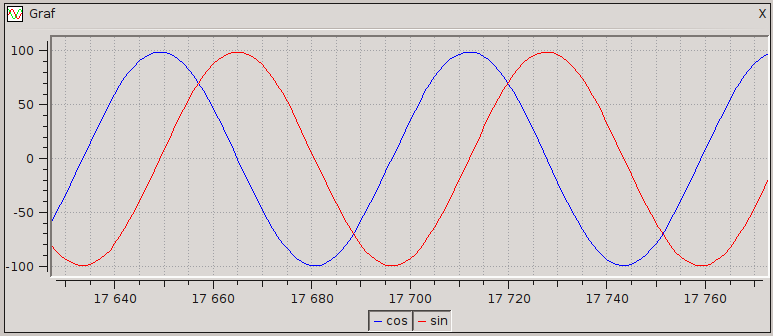
\includegraphics[scale=0.65]{img/w_graph.png}
\caption{Widget: graf}
\end{center}
\end{figure}
Widget graf zobrazuje hodnoty v grafu -- na osu $x$ se vynáší pořadí dat a na osu $y$ hodnoty dat. Lze nastavovat jméno, barvu a datový typ křivky grafu, automatické posouvání grafu, velikost vzorku, měřítko os grafu a zobrazení legendy. Kliknutí na křivku grafu v legendě tuto křivku skryje. Měřítko osy se ovládá otáčením kolečka myši po najetí kurzoru nad osu, po najetí do prostoru grafu se podobně ovládá měřítko celého grafu. 
\begin{figure}[h]
\begin{center}
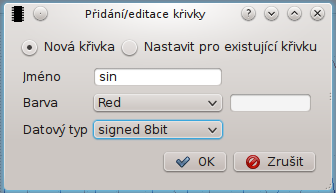
\includegraphics[scale=0.8]{img/w_graph_add.png}
\caption{Dialog pro nastavení parametrů křivky grafu}
\end{center}
\end{figure}

%\newpage
\subsection{Widget: script}
%\addcontentsline{toc}{subsection}{Widget: script}
\begin{figure}[h]
\begin{center}
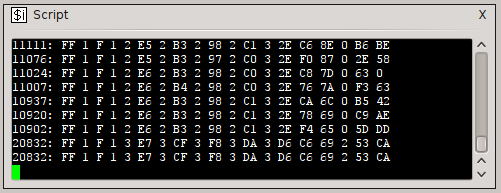
\includegraphics[scale=0.8]{img/w_script.png}
\caption{Widget: script}
\label{script_w}
\end{center}
\end{figure}
Tento widget umožňuje zpracovávání dat pomocí scriptu, který si napíše sám uživatel. Jazyk, ve kterém se tento script píše je QtScript\cite{qtscript} (jazyk založený na standartu ECMAScript\footnote{\It{ECMAScript} -- scriptovací jazyk stadartu ECMA-262 a ISO/IEC 16262}, stejně jako JavaScript\footnote{\It{JavaScript} -- objektově orientovaný skriptovací jazyk, používaný hlavně na webu}, díky tomu jsou tyto jazyky velmi podobné). Script může zpracovávat příchozí data, reagovat na stisky kláves a posílat data do zařízení. Základní výstup může být zobrazen v terminálu (viz obrázek \ref{script_w}), je však možné využít ke zobrazování také ostatní widgety (číslo, bar, ...) -- script si je vytvoří jako objekt a nastavuje do nich data. Reference k vestavěným funkcím, které lze použít ve scriptu, je v \hyperref[script_ref]{příloze A}.
%DOP: že umožní zprcování hodně typů dat?
%TODO Qtscript ref
\begin{figure}[h]
\begin{center}
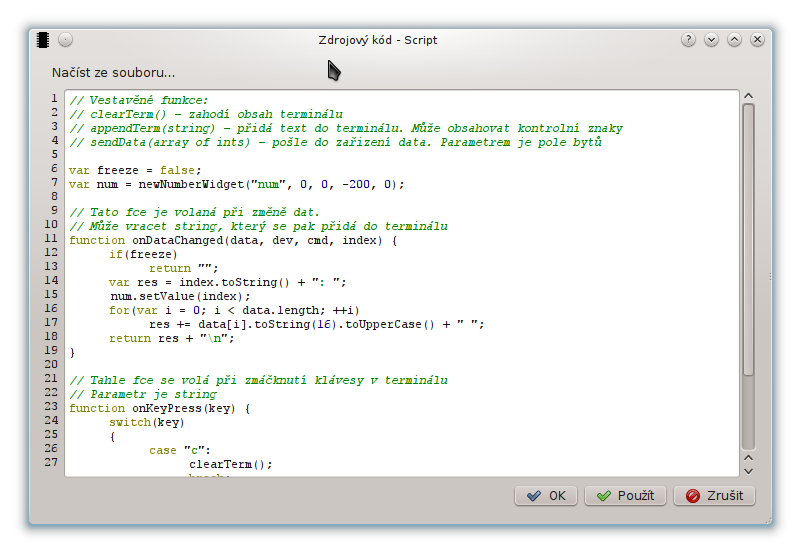
\includegraphics[width=\textwidth]{img/w_script_src.png}
\caption{Dialog pro nastavení zdrojového scriptu}
\end{center}
\end{figure}

\newpage
\setlength{\voffset}{0mm} % posune text/obrázek na této stránce, kam patøí
\pagestyle{plain}

\section{Modul: Proxy mezi sériovým portem a TCP socketem}
%\addcontentsline{toc}{section}{Modul: Proxy mezi sériovým portem a TCP socketem} 
%\addcontentsline{toc}{subsection}{Popis}

\begin{figure}[H]
\begin{center}
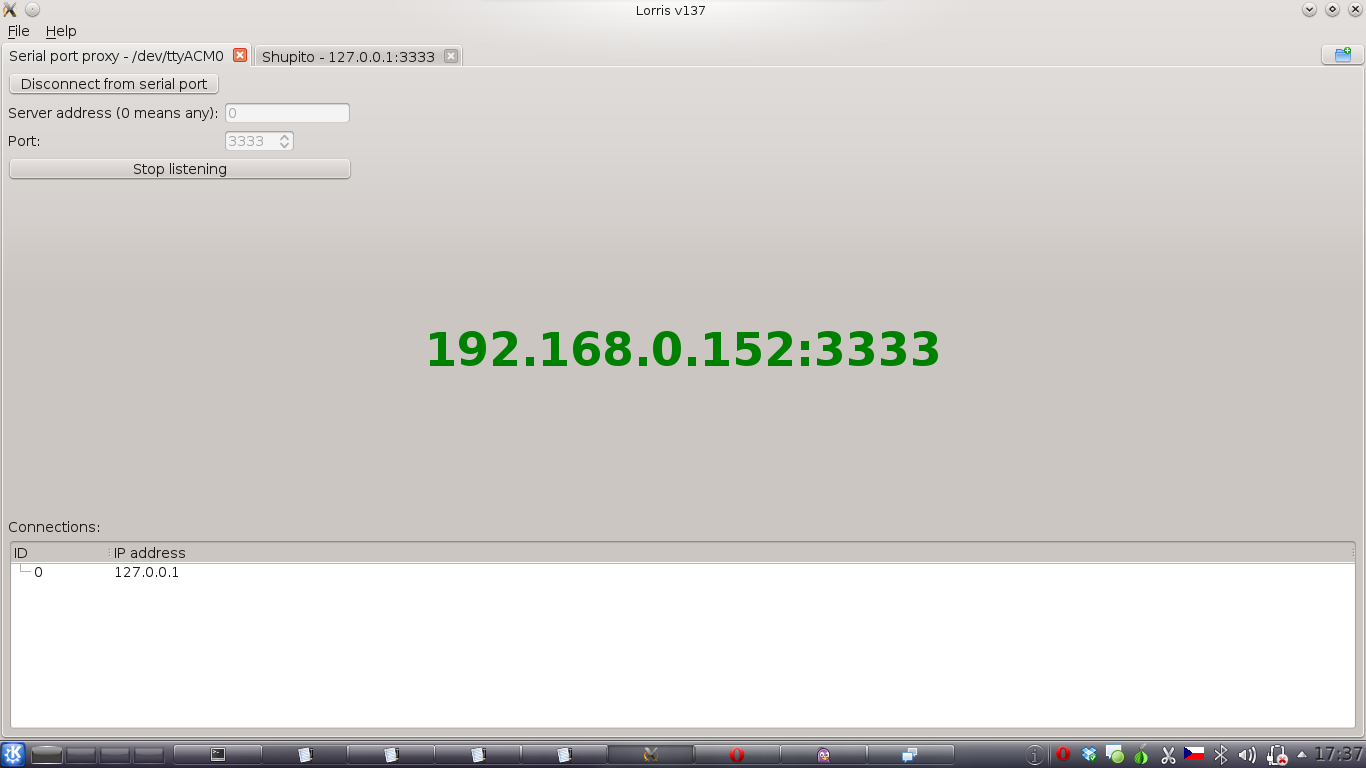
\includegraphics[width=\textwidth]{img/proxy.png}
\caption{Proxy mezi sériovým portem a TCP socketem}
\label{Shupito}
\end{center}
\end{figure}
Jednoduchá proxy mezi sériovým portem a TCP socketem. Vytvoří server, na který je možné se připojit z Lorris nebo jiného programu na jiném počítači. Po připojení se přeposílají data ze sériového portu připojeným klientům a naopak.

\newpage
\setlength{\voffset}{0mm} % posune text/obrázek na této stránce, kam patøí
\pagestyle{plain}

\section{Modul: Shupito}
%\addcontentsline{toc}{section}{Modul: Shupito} 
%\addcontentsline{toc}{subsection}{Popis}

\begin{figure}[h]
\begin{center}
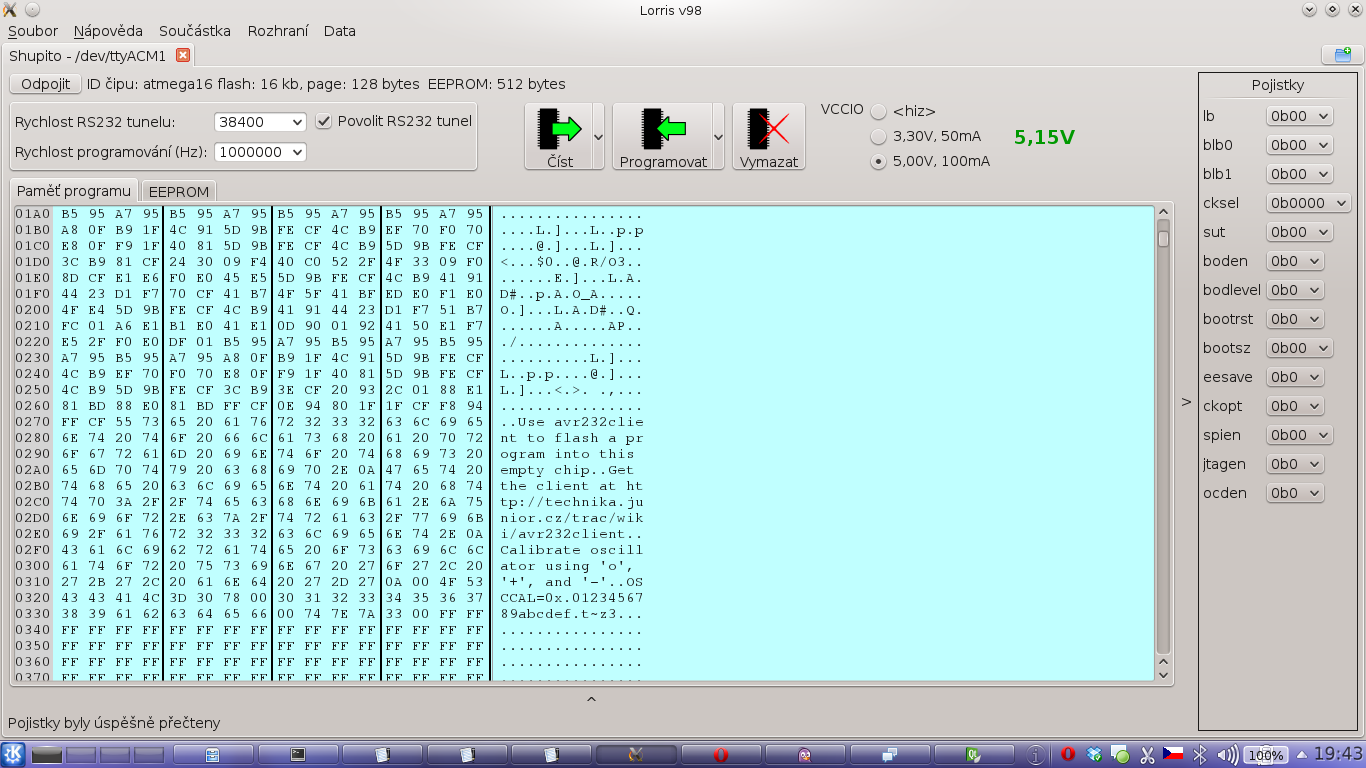
\includegraphics[width=\textwidth]{img/shupito.png}
\caption{Modul Shupito}
\label{Shupito}
\end{center}
\end{figure}
% DOP: popsat typy programováni
Shupito je programátor mikročipů vytvořený Martinem Vejnárem, který dokáže programovat mikrokontroléry pomocí ISP\footnote{\It{In-system programming} -- rozhraní, které umožňuje programovat čipy bez dalšího zařízení přímo v desce plošného spoje.}, PDI\footnote{\It{Program and Debug Interface} -- rozhraní firmy Atmel umožňující programování čipů přímo na desce, podobně jako ISP} a JTAG\footnote{\It{Joint Test Action Group} -- rozhraní podle standartu IEEE 1149.1 umožňující mimo jiné programování a debugování čipů} rozhraní. 

% DOP: opravit
Modul v mojí práci dokáže obsluhovat programátor Shupito -- nastavovat výstupní napětí, číst a programovat paměť čipů (flash i EEPROM) a číst a měnit pojistky. Jako výstupní i vstupní data používá soubory ve formátu Intel HEX32\footnote{\It{Intel HEX32} -- formát souborů obsahující paměť čipu}. 
Způsob komunikace s programátorem je přenesen z oficiálního ovládacího programu\cite{avr232client}, který je však na rozdíl od Lorris dostupný pouze pro MS Windows.

\subsection{RS232 tunel}
%\addcontentsline{toc}{subsection}{RS232 tunel}
\label{tunel}
Shupito dokáže vytvořit tunel\footnote{Přímé spojení programovaného čipu a počítače přes programátor.} pro RS232 linku z programovaného čipu do počítače. Lorris umí této funkce využít -- aktivní tunel se zobrazí jako další typ připojení a je možné se na něj připojit v ostatních modulech.

\begin{figure}[H]
\begin{center}
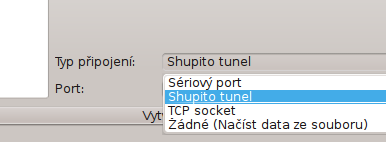
\includegraphics{img/con_tunel.png}
\caption{Možnost Shupito Tunel v dialogu připojení k zařízení}
\end{center}
\end{figure}

\newpage
\section{Modul: Terminál}
%\addcontentsline{toc}{section}{Modul: Terminál} 
%\addcontentsline{toc}{subsection}{Popis}

\begin{figure}[h]
\begin{center}
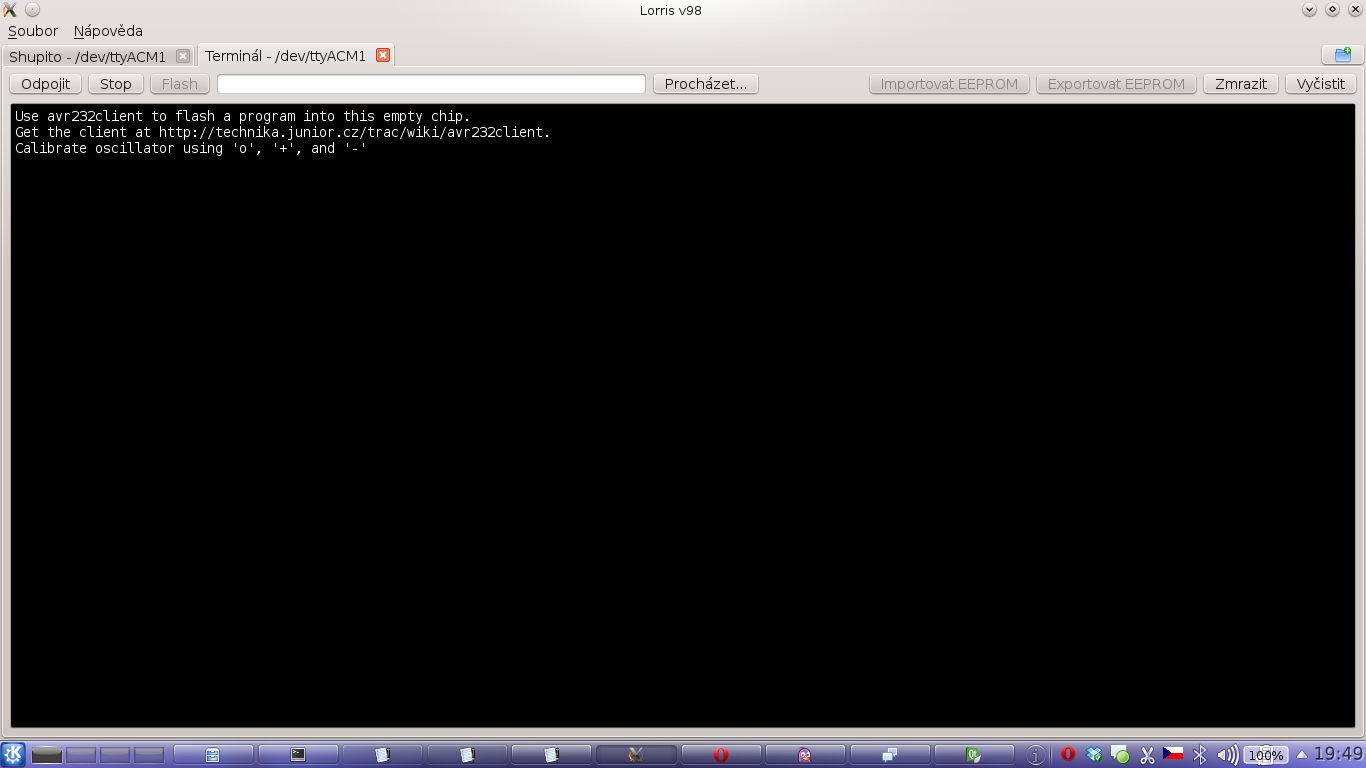
\includegraphics[width=\textwidth]{img/terminal.png}
\caption{Modul terminál}
\label{Terminal}
\end{center}
\end{figure}

Klasický terminál -- zobrazuje data přijatá přes sériový port a posílá stisky kláves. Je obohacený o podporu bootloaderu pro mikrokontroléry AVR ATmega (bootloader byl taktéž napsaný Martinem Vejnarem), který umožňuje jejich programování přes RS232 linku. Informace o protokolu bootloaderu jsem získal z oficiálního programu určeného k programování přes tento bootloader, avr232client.


\newpage
\section{Příklady použití}
%\addcontentsline{toc}{section}{Příklady použití}
\subsection{Testování barevného senzoru}
%\addcontentsline{toc}{subsection}{1. Testování barevného senzoru}
{\bf Situace:} Stavím robota do soutěže (Eurobot, RobotChallange, ...), ve které je možné se na herním poli orientovat podle barvy. Chci barevný senzor otestovat, proto jsem na nepájivém poli postavil jednoduchý obvod s čipem, na který je senzor připojený. Čip bude dávat senzoru pokyny k měření a vyčítat z něj RGB hodnoty, které následně pošle do RS232 linky.\\
\\
{\bf Řešení:} Program, který bude ze senzoru číst hodnoty naprogramuji do čipu pomocí programátoru Shupito, který také poskytne tunel pro RS232 linku. Na tento tunel se připojím modulem Analyzér, ve kterém díky widgetu \uv{barva} mohu vidět barvu, kterou senzor rozpoznal.

\begin{figure}[h]
\begin{center}
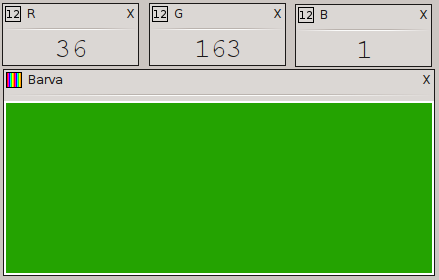
\includegraphics{img/use_color.png}
\caption{Barva v modulu Analyzér}
\label{Terminal}
\end{center}
\end{figure}

\newpage
\subsection{Testování enkodérů}
%\addcontentsline{toc}{subsection}{2. Testování enkodérů}
{\bf Situace:} Potřebuji otestovat přesnost magnetických enkodérů, které však odesílají data o úhlu natočení rozdělené v několika bytech v takovém formátu, který znemožňuje použití např. terminálu.\\
\\
{\bf Řešení:} Nechci za tímto účelem stavět a programovat novou desku s dalším mikročipem, připojím tedy enkodér k počítači. V Lorris otevřu modul analyzér a ve widgetu \uv{script} napíši  jednoduchý script, který složí úhel do jednoho čísla a zobrazí ho ve widgetu \uv{číslo}.

\begin{figure}[H]
\begin{center}
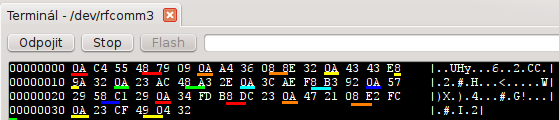
\includegraphics{img/use_enc_term.png}
%DOP y/i?
\caption{Surová data z enkodérů s vyznačenými byty, které obsahují úhel natočení}
\label{Terminal}
\end{center}
\end{figure}

\begin{figure}[H]
\begin{center}
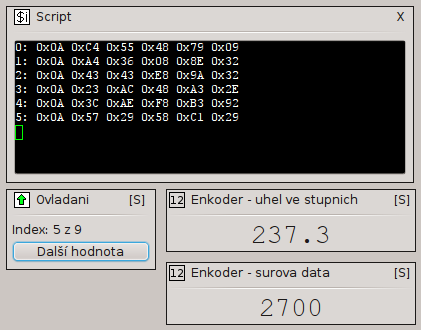
\includegraphics{img/use_enc_analyzer.png}
\caption{Data z enkodérů zpracovaná analyzérem}
\label{Terminal}
\end{center}
\end{figure}

\newpage
\subsection{Ladění PID regulátoru}
%\addcontentsline{toc}{subsection}{3. Ladění PID regulátoru}
{\bf Situace:} Robot kvůli rozdílnému výkonu motorů nejede rovně. Tento problém jsem se rozhodl řešit pomocí PID regulátoru, pro jehož správnou funkci je potřeba nastavit několik konstant. \\
\\
{\bf Řešení:} Program v robotovi mi posílá aktualní výkon motorů a nastavení konstant PID regulátoru a umožňuje přenastavení těchto konstant a ovládání robota. Tento program do robota nahrávám přes bluetooth pomocí modulu Terminál, protože čip má v sobě bootloader -- díky tomu nemusím mít připojený programátor.  

V modulu analyzér si zobrazím aktuální hodnoty PID regulátoru (jako číslo) a výkon motorů (jako graf či číslo). Do widgetu script napíši jednoduchý script, který po stisku kláves změní nastavení konstant regulátoru nebo rozjede/zastaví robota.

%refg
Tento postup jsem použil při ladění PID regulátoru robota 3pi\cite{3pi} během přípravy na soutěž \It{Line Follower Standard}, která je součástí Robotického dne 2012\cite{rob_den}.
\begin{figure}[H]
\begin{center}
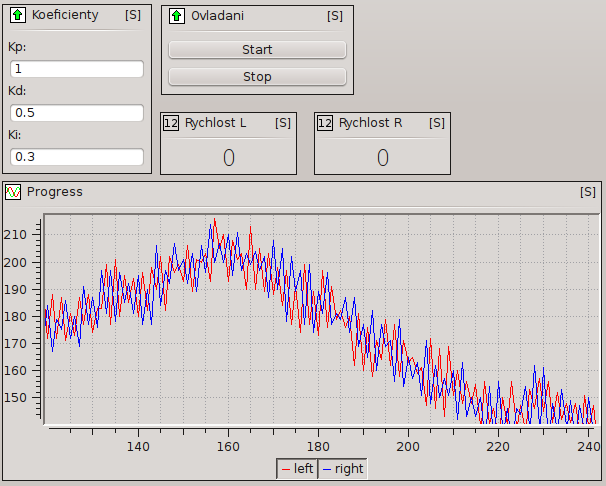
\includegraphics[scale=0.55]{img/use_pid.png}
\caption{Ladění PID regulátoru}
\end{center}
\end{figure}

\newpage
\subsection{Vývoj robota pro soutěž Eurobot 2011}
%\addcontentsline{toc}{subsection}{4. Vývoj robota pro soutěž Eurobot 2011}
V minulém roce jsem se zúčastnil soutěže Eurobot\cite{eurobot}. Cíl soutěže je každý rok jiný, v minulém ročníku bylo cílem hrát něco jako zjednodušené šachy. Herní hřiště bylo rozděleno na barevnou šachovnici a leželi na něm \uv{pěšci} (žluté disky), které měli roboti posouvat na políčka svojí barvy, případně z nich stavět věže. Vyhrával robot s největším počtem bodů, které získával za pěšce na polích svojí barvy a postavené věže. Roboti navíc musí mít vyřešenou detekci soupeře, aby do sebe nenaráželi (např. pomocí ultrazvukových měřičů vzdálenosti). Kompletní pravidla, výsledková listina a další informace jsou na webu ročníku 2011\cite{eurobot11}.

Robot našeho týmu byl poměrně jednoduchý, přesto však obsahoval 5 ultrazvukových měřáků vzdálenosti, dva enkodéry a 5 tlačítek (detekce nárazu na mantinel a pěšce, kterého mohl robot převážet). Tyto senzory produkují poměrně značné množství dat, které se v terminálu zobrazuje nepřehledně.

\begin{figure}[H]
\begin{center}
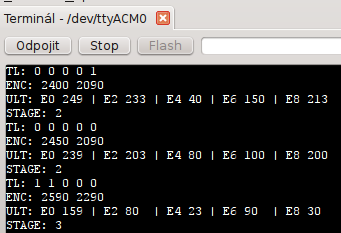
\includegraphics{img/use_david1.png}
\caption{Data z robota v terminálu}
\end{center}
\end{figure}

Zkušenost s programováním a laděním robota byla jedním z hlavních důvodů pro výběr zvoleného tématu práce. S použitím programu Lorris by se mohla tato data zobrazovat například takto:
\begin{figure}[H]
\begin{center}
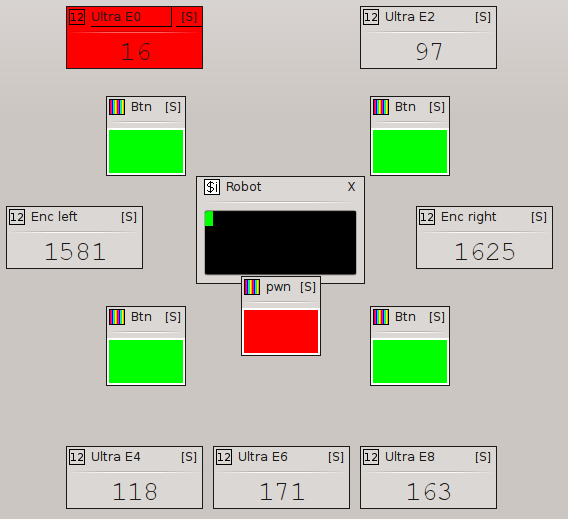
\includegraphics{img/use_david2.png}
\caption{Simulovaná data v analyzéru}
\end{center}
\end{figure}

Všechny widgety jsou rozmístěné stejně jako na robotovi -- 2 ultrazvuky měří vzdálenost vepředu, 3 vzadu; tlačítka pro detekci mantinelu jsou na každém rohu, tlačítko uvnitř robota ověřuje,  zda robot nabral pěšce a enkodéry na obou kolech měří ujetou vzdálenost.

Widget \It{script} s názvem \uv{Robot} uprostřed reprezentuje tělo robota. Widgety \It{číslo} s názvy \uv{Ultra E0...8} ukazují vzdálenost z ultrazvukových měřáků. Ve widgetu \uv{Ultra E0} je vzdálenost menší než 25 cm, což je hraniční vzdálenost, po které se robot zastaví, aby nevrazil do soupeře -- aby widget na tuto skutečnost upozornil, má červené pozadí.

Widgety \It{barva} s názvy \uv{btn} jsou tlačítka značící náraz do mantinelu a \uv{pwn} je tlačítko, které se stiskne, pokud je v robotovi pěšec. Tlačítko, které má zelenou barvu, není stisklé, tlačítko s červenou barvou stisklé je.

Poslední widgety \It{číslo} s názvy \uv{Enc left} a \uv{Enc right} vypisují ujetou vzdálenost z enkodérů pravého a levého kola.

\begin{figure}[H]
\begin{center}
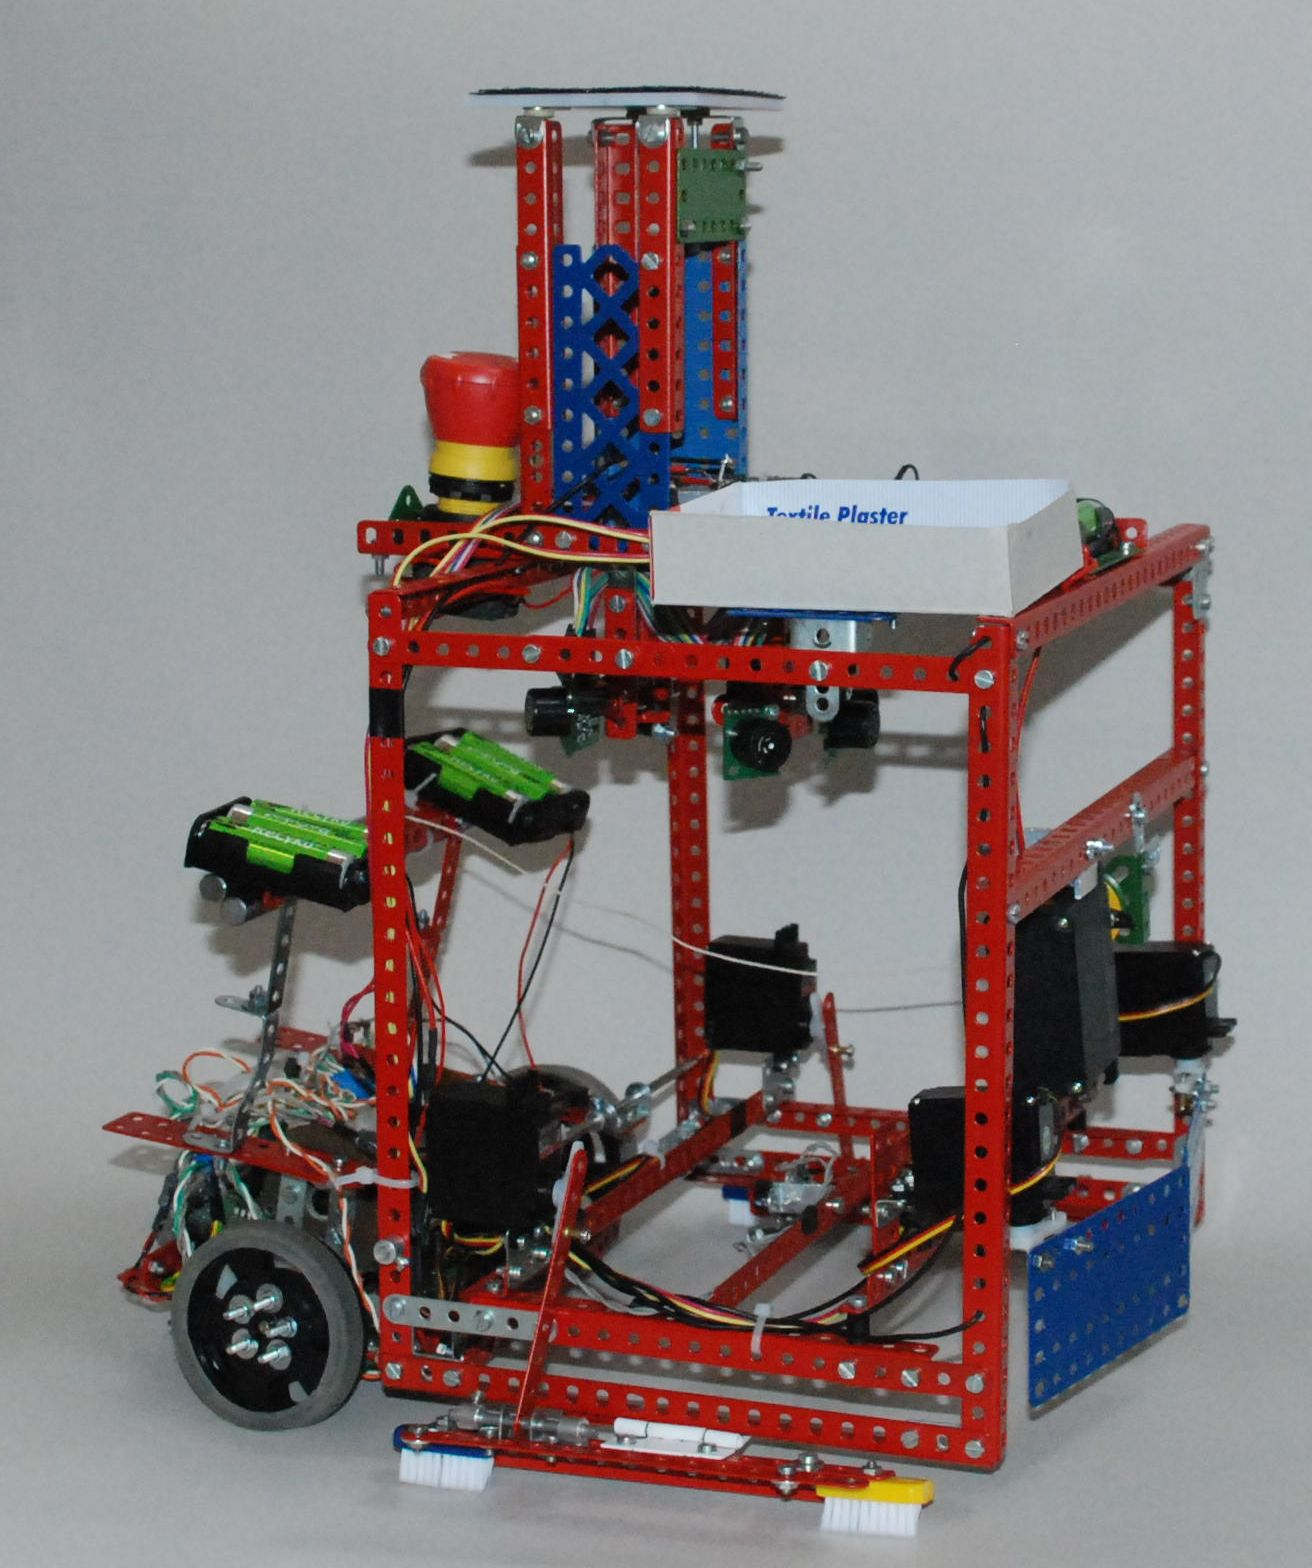
\includegraphics[scale=0.24]{img/use_david_robot.jpg}
\caption{Náš robot \It{David} skončil na 4. místě v celostátním kole soutěže Eurobot 2011}
\end{center}
\end{figure}

\newpage
\section*{Závěr}
\addcontentsline{toc}{section}{Závěr}
Vytvořená aplikace splňuje všechny stanovené požadavky:
\begin{enumerate}[label=\Has\hspace{1.5mm}\arabic{*}.]
    \item Možnost zpracovávat data přicházející ze zařízení a přehledně je zobrazovat% 1
    \item Podpora co nejvíce formátů příchozích dat% 2
    \item Snadné a rychlé používání % 3
    \item Možnost běhu i na jiných systémech než je MS Windows % 4
    \item Co možná nejnižší cena -- program je dostupný zdarma% 5
    \item Snadná rozšířitelnost (ideálně otevřený zdrojový kód) % 6
    \item Nezávislost na další aplikaci (např. MS Office Excel) % 7
\end{enumerate}
Program navíc výrazně přesáhl původní cíle -- mimo zobrazování dat dokáže posílat data i zpět do zařízení, programovat mikročipy a vytvořit proxy mezi sériovým portem a TCP socketem. Ve srovnání s~nalezenými programy s~podobným zaměřením (viz úvod) je také jediný, který umožňuje uživateli napsat vlastní script pro parsování dat.

Přestože se jedná o zcela nový software, byl již použit při testování barevného senzoru, ladění PID regulátoru pro robota na sledování čáry a je používán pro ovládání programátoru Shupito. Další možnosti použití jsou uvedeny v kapitole 6.

Aplikace je nadále vyvíjena, mohu prakticky donekonečna přídávat buďto další typy widgetů do modulu Analyzér (například kompas, směrový kříž, ...) nebo celé nové moduly (například ovládání robota pomocí joysticku). Program má v současné době (19.4.2012) asi 15 a půl tisíce řádků kódu (bez knihoven třetích stran). Zdrojové kódy a instruktážní video jsou přiloženy na CD. 
\begin{figure}[H]
\begin{center}
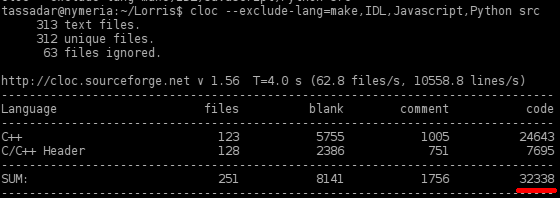
\includegraphics[width=\textwidth]{img/cloc_edit.png}
\caption{Počet řádků spočítaný programem CLOC\cite{cloc}}
\end{center}
\end{figure}

Kromě přidávání dalších vlastností do tohoto programu bych v budoucnu rád vytvořil podobný program (hlavně vlastnosti modulu Analyzér) pro přenosná zařízení (chytrý mobilní telefon či tablet), protože pro tato zařízení žádná taková aplikace v současné době neexistuje a chtěl bych vyzkoušet programování pro tyto platformy (zejména pro Google Android\cite{android}).

%%%%%%%%%%%%%%%%%%%%%%%%%%%%%%%%%%%%%%%%%%%%%%%%%%%%%%%%%%%%%%%%%%%%%%%%%%%
\newpage

%\section*{PŘÍLOHY}
%\addcontentsline{toc}{section}{PŘÍLOHY}

\section*{PŘÍLOHA A:}
\section*{Reference k widgetu \It{script}}
\addcontentsline{toc}{section}{PŘÍLOHA A: Reference k widgetu \It{script}}
\label{script_ref}
Widget \It{script} umožňuje parsování dat pomocí scriptu, který se píše v QtScriptu, který je založený na standartu ECMAScript, na kterém je založený JavaScript. Jazyk je hodně podobný JavaScriptu a většinou můžete použít jeho referenci. Tento text předpokládá alespoň základní znalost JavaScriptu nebo podobného programovacího jazyku.

\begin{itemize}
    \item \url{http://en.wikipedia.org/wiki/ECMAScript}
    \item \url{https://qt-project.org/doc/qt-4.8/scripting.html}
    \item \url{http://www.w3schools.com/jsref/default.asp} -- JS reference
\end{itemize}

\subsection*{Základní script}
\addcontentsline{toc}{subsection}{Základní script}
Script by měl obsahovat následující dvě funkce (ale nemusí, pokud je nepoužívá):

\noindent\begin{minipage}{\textwidth}
\begin{lstlisting}[caption=Základní script]
function onDataChanged(data, dev, cmd, index) {
    return "";
}

function onKeyPress(key) {

}
\end{lstlisting}
\end{minipage}

{\color{blue}\verb/onDataChanged(data, dev, cmd, index)/} je volána při změně pozice v datech (tj. když přijdou nová data nebo uživatel pohne posuvníkem historie). Může vracet \verb/string/, který se přidá do terminálu.

\begin{itemize}
    \item \verb/data/ -- {\bf pole s Integery} obsahující příchozí data
    \item \verb/dev/ -- {\bf Integer} s ID zařízení (může být definováno v hlavičce packetu -- pokud není, \verb/dev/ se rovná -1)
    \item \verb/cmd/ -- {\bf Integer} s ID příkazu (může být definováno v hlavičce packetu -- pokud není, \verb/cmd/ se rovná -1)
    \item \verb/index/ -- {\bf Integer} s indexem packetu v příchozích datech.
\end{itemize}

{\color{blue}\verb/onKeyPress(key)/} je volána po stisku klávesy v terminálu. Tato funkce by neměla vracet nic.
\begin{itemize}
    \item \verb/key/ -- {\bf String} se stisknutou klávesou
\end{itemize}

\subsection*{Dostupné funkce}
\addcontentsline{toc}{subsection}{Dostupné funkce}
Jsou dostupné základní javascriptové knihovny (\verb/Math/, \verb/Date/, ...) a samotný Lorris poskytuje další rozšiřující funkce. 

\begin{itemize}
    \item {\color{blue}\verb/appendTerm(string)/} -- přidá do terminálu text.\\
        \noindent\begin{minipage}{\textwidth}
        \begin{lstlisting}[caption=Vypsání stisknutých kláves do terminálu]
function onKeyPress(key) {
    appendTerm(key); // vypise _key_ do terminalu
}
        \end{lstlisting}
        \end{minipage}

    \item {\color{blue}\verb/clearTerm()/} -- vyčistí terminál.\\
        \noindent\begin{minipage}{\textwidth}
        \begin{lstlisting}[caption=Vypsání stisknutých kláves do terminálu a jeho vyčištění po stisku klávesy C]
function onKeyPress(key) {
    if(key == "c")
        clearTerm(); // vycisti terminal
    else
        appendTerm(key); // vypise _key_ do terminalu
}
        \end{lstlisting}
        \end{minipage}

    \item {\color{blue}\verb/sendData(pole Integerů)/} -- pošle data do zařizení\\
        \noindent\begin{minipage}{\textwidth}
        \begin{lstlisting}[caption=Poslání ASCII kódu stisknuté klávesy]
function onKeyPress(key) {
    sendData(new Array(key.charCodeAt(0)));
}
        \end{lstlisting}
        \end{minipage}

    \item {\color{blue}\verb/newXXXXWidget()/} -- tato funkce potřebuje o něco obsáhlejší popis, který je v následující kapitole
\end{itemize}

\subsection*{Vytvoření widgetu}
\addcontentsline{toc}{subsection}{Vytvoření widgetu}

Script může vytvořit všechny ostatní typy widgetů a posílat do nich data. Samotných funkcí je několik, každá vytvoří jiný typ widgetu:
\begin{itemize}
    \item {\color{blue}\verb/newNumberWidget(...)/} -- vytvoří widget \It{číslo}
    \item {\color{blue}\verb/newBarWidget(...)/} -- vytvoří widget \It{sloupcový bar}
    \item {\color{blue}\verb/newColorWidget(...)/} -- vytvoří widget \It{barva}
    \item {\color{blue}\verb/newGraphWidget(...)/} -- vytvoří widget \It{graf}
    \item {\color{blue}\verb/newInputWidget(...)/} -- vytvoří widget \It{vstup} (dostupný pouze ze scriptu)
\end{itemize}

Všechny tyto funkce mají stejné parametry a vrací object widgetu.
{\color{blue}
\begin{verbatim}newXXXXWidget("jméno");
newXXXXWidget("jméno", šířka, výška);
newXXXXWidget("jméno", šířka, výška, Xoffset, Yoffset);
\end{verbatim}
}

\begin{itemize}
    \item \verb/jméno/ -- {\bf String}, jméno widgetu, zobrazí se v titulku
    \item \verb/šířka/ -- {\bf Integer}, šířka widgetu v pixelech. Může být 0, poté se zvolí minimální velikost.
    \item \verb/výška/ -- {\bf Integer}, výška widgetu v pixelech. Může být 0, poté se zvolí minimální velikost.
    \item \verb/Xoffset/ -- {\bf Integer}, vodorovná vzdálenost v pixelech od levého horního rohu mateřského ScriptWidgetu. Může být 0, widget se poté vytvoří v levém horním rohu aktuálně viditelné plochy.
     \item \verb/Yoffset/ -- {\bf Integer}, svislá vzdálenost v pixelech od levého horního rohu mateřského ScriptWidgetu. Může být 0, widget se poté vytvoří v levém horním rohu aktuálně viditelné plochy.
\end{itemize}

\noindent\begin{minipage}{\textwidth}
\begin{lstlisting}[caption=Vytvoření widgetu \It{číslo} a nastavení jeho hodnoty z příchozích dat]
var cislo = newNumberWidget("rychlost", 200, 100, -250, 0);

function onDataChanged(data, dev, cmd, index) {
    cislo.setValue(data[0]);
    return "";
}
\end{lstlisting}
\end{minipage}

\subsection*{Dostupné funkce widgetů}
\addcontentsline{toc}{subsection}{Dostupné funkce widgetů}
Objekt widgetu je podtřídou třídy z Qt Frameworku QWidget -- díky tomu může používat jeho vlastnosti a sloty. Popis vlastností najdete v Qt referenci\footnote{\url{http://qt-project.org/doc/qt-4.7/qwidget.html\#propertySection}} v kapitole \uv{Properties} a ve scriptu se používají takto:

\noindent\begin{minipage}{\textwidth}
\begin{lstlisting}[caption=Vytvoření widgetu \It{číslo} a nastaveni vlastnosti \uv{width}]
var cislo = newNumberWidget("rychlost", 200, 100, -250, 0);
cislo.width = 40; // nastaveni sirky widgetu
\end{lstlisting}
\end{minipage}

Popis slotů je taktéž v Qt referenci, tentokrát pod kapitolou \uv{Public slots}. Používají se jako metody:

\noindent\begin{minipage}{\textwidth}
\begin{lstlisting}[caption=Vytvoření widgetu \It{číslo} a použití slotu]
var cislo = newNumberWidget("rychlost", 200, 100, -250, 0);
cislo.setDisabled(true); // znemozneni interakce s widgetem
\end{lstlisting}
\end{minipage}

Kromě těchto zděděných vlastností a funkcí má každý typ widgetu své vlastní.

%\newpage
\subsubsection*{Widget číslo}
\addcontentsline{toc}{subsubsection}{Widget číslo}
\begin{itemize}
    \item {\color{blue}\verb/setValue(Integer nebo double)/} -- Nastaví hodnotu widgetu
\end{itemize}

\noindent\begin{minipage}{\textwidth}
\begin{lstlisting}[caption=Nastavení hodnoty widgetu \It{číslo}]
var cislo = newNumberWidget("test cislo", 200, 100, -250, 0);
cislo.setValue(40);
...
cislo.setValue(3.14);
\end{lstlisting}
\end{minipage}

\subsubsection*{Widget sloupcový bar}
\addcontentsline{toc}{subsubsection}{Widget sloupcový bar}
\begin{itemize}
    \item {\color{blue}\verb/setValue(Integer)/} -- Nastaví hodnotu widgetu
    \item {\color{blue}\verb/setRange(Integer min, Integer max)/} -- Nastaví minimální a maximální hodnotu widgetu
    \item {\color{blue}\verb/rotationSelected(Integer)/} -- Nastaví rotaci sloupce. 0 pro svislou, 1 pro vodorovnou
\end{itemize}

\noindent\begin{minipage}{\textwidth}
\begin{lstlisting}[caption=Nastavení hodnot widgetu \It{sloupcový bar}]
var bar = newBarWidget("test bar");
bar.setRange(0, 100); // rozmezi hodnot 0 az 100
bar.setValue(45); // nastaveni hodnoty na 45
bar.rotationSelected(1); // otoceni na vodorovno
\end{lstlisting}
\end{minipage}

\subsubsection*{Widget barva}
\addcontentsline{toc}{subsubsection}{Widget barva}
\begin{itemize}
    \item {\color{blue}\verb/setValue(Integer r, Integer g, Integer b)/} -- Nastaví barvu z hodnot RGB (každá 0 až 255)
    \item {\color{blue}\verb/setValue(String barva)/} -- Nastaví barvu z hex hodnoty jako v HTML (např. \#FF0000 pro červenou)
\end{itemize}

\noindent\begin{minipage}{\textwidth}
\begin{lstlisting}[caption=Nastavení hodnot widgetu \It{barva}]
var bar = newColorWidget("test barva");
bar.setValue(255, 255, 0);
...
bar.setValue("#00FF00");
\end{lstlisting}
\end{minipage}

\subsubsection*{Widget graf}
\addcontentsline{toc}{subsubsection}{Widget graf}
Tento widget se od ostatních poměrně výrazně liší -- je třeba nejdříve vytvořit křivku až té nastavovat hodnoty. Funkce samotného widgetu graf jsou tyto:
\begin{itemize}
    \item {\color{blue}\verb/addCurve(String jméno, String barva)/} -- Vytvoří a vrátí novou křivku. \verb/barva/ může být buďto html název (např. red, blue) nebo HTML hex zápis (např. \#FF0000)
    \item {\color{blue}\verb/setAxisScale(bool proX, double min, double max)/} -- Nastaví měřítko os. \verb/proX/ je {\bf true} pokud nastavujete měřítko osy $x$
    \item {\color{blue}\verb/updateVisibleArea()/} -- Přesune pohled na nejvyšší hodnotu osy $x$
\end{itemize}

{\color{blue}\verb/addCurve(String jméno, String barva)/} vrátí křivku, která má tyto funkce:

\begin{itemize}
    \item {\color{blue}\verb/addPoint(Integer index, double hodnota)/} -- Vloží bod křivky. \verb/index/ určuje pořadí bodů (bod s indexem 0 bude vždy před bodem s indexem 50, i když bude vložen až po něm). Pokud bod se stejným indexem už existuje, je jeho hodnota změněna
    \item {\color{blue}\verb/clear()/} -- Smaže všechny body křivky
\end{itemize}

\noindent\begin{minipage}{\textwidth}
\begin{lstlisting}[caption=Zobrazení křivky funkce sinus ve widgetu \It{graf}]
var graf = newGraphWidget("graf", 400, 250, -420, 0);
graf.setAxisScale(false, -105, 105); // meritko osy y
graf.setAxisScale(true, 0, 200); // meritko osy x

// vytvoreni krivky sin
var sin = graf.addCurve("sin", "blue"); 

// pridani bodu do krivky sin
var sinVal = 0;
for(var i = 0; i < 500; ++i)
{
    sin.addPoint(i, Math.sin(sinVal)*100);
    sinVal += 0.1;
}
// presunuti na posledni hodnotu krivky
graf.updateVisibleArea(); 
\end{lstlisting}
\end{minipage}

\subsubsection*{Widget vstup}
\addcontentsline{toc}{subsubsection}{Widget vstup}
Tento widget lze vytvořit pouze ze scriptu a umí zobrazit a ovládat většinu Qt widgetů\footnote{\url{http://qt-project.org/doc/qt-4.7/widgets-and-layouts.html}}, například tlačítko (\verb/QPushButton/), zaškrtávací políčko (\verb/QCheckBox/) či textové políčko (\verb/QLineEdit/). Dokumentace k těmto widgetům je v Qt referenci, opět můžete používat vlastnosti (\uv{Properties}) a funkce (\uv{Public slots}).\\
Funkce widgetu \It{vstup}:
\begin{itemize}
    \item {\color{blue}\verb/newWidget(String jméno, Integer roztahování = 0)/} -- Vytvoří a vrátí nový QWidget. \verb/jméno/ musí být jméno třídy widgetu, například QPushButton, QCheckBox nebo QLineEdit. \verb/roztahování/ značí jak moc se bude widget roztahovat oproti ostatním.
\end{itemize}


\noindent\begin{minipage}{\textwidth}
\begin{lstlisting}[caption=Widget \It{vstup} -- vytvoření QLabel]
var vstup = newInputWidget("test vstupu", 150, 100, -160, 0);
var label = vstup.newWidget("QLabel", 1);

// zarovnani textu na stred. 
// 0x0080 a 0x0004 jsou konstanty Qt Frameworku 
// Qt::AlignHCenter a Qt::AlignVCenter
label.alignment = 0x0080 | 0x0004;

// nastaveni textu
label.text = "Testovaci popisek";
\end{lstlisting}
\end{minipage}

Widget vytvořený tímto příkladem vypadá takto:

\begin{figure}[H]
\begin{center}
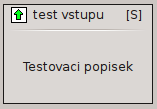
\includegraphics{img/ref_input.png}
\caption{Widget \It{vstup} -- vytvoření QLabel}
\end{center}
\end{figure}

\newpage
QtScript podporuje i využití principu signálů a slotů, díky tomu lze ve scriptu reagovat například na stisknutí tlačítka.

\noindent\begin{minipage}{\textwidth}
\begin{lstlisting}[caption=Widget \It{vstup} -- tlačítko]
var vstup = newInputWidget("test vstupu", 150, 100, -160, 0);

var rychlost = vstup.newWidget("QLineEdit");
rychlost.text = "100";

var btn = vstup.newWidget("QPushButton", 1);
btn.text = "Nastavit";

function posliRychlost()
{
    var speed = parseInt(rychlost.text);
    sendData(new Array(speed));
    appendTerm("Rychlost " + speed + "odeslana\n");
}
// Pripojeni signalu "clicked" na slot posliRychlost()
btn.clicked.connect(posliRychlost);
\end{lstlisting}
\end{minipage}

\begin{figure}[H]
\begin{center}
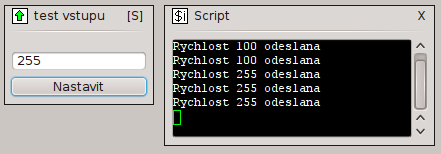
\includegraphics{img/ref_input2.png}
\caption{Widget \It{vstup} -- tlačítko}
\end{center}
\end{figure}

\subsection*{Pár věcí, na které je třeba při programování myslet}
\addcontentsline{toc}{subsection}{Pár věcí na které je třeba myslet}
\begin{itemize}
    \item Widgety vytvořené ze scriptu se neukládájí do datového souboru -- po načtení se vytvoří znovu, bez dat.
    \item Stav proměnných ve scritptu se zatím neukládá do souboru.
    \item Po stisknutí \uv{Ok} nebo \uv{Použít} v dialogu nastavení scritpu se script načte znovu -- staré widgety se smažou a vytvoří nové, bez dat.
    \item Jazyk nemá žádné pojistky proti \uv{špatnému} kódu -- pokud ve scritpu bude nekonečná smyčka, Lorris prostě zamrzne
\end{itemize}

\newpage
\section*{PŘÍLOHA B:}
\section*{Knihovny třetích stran}
\addcontentsline{toc}{section}{PŘÍLOHA B: Knihovny třetích stran}
\begin{itemize}
    \item {\bf Qwt}\cite{qwt} je knihovna pro Qt Framework obsahující tzv. widgety pro aplikace technického charakteru -- grafy, sloucové ukazatele, kompasy a podobně. Ve svojí práci zatím z této knihovny používám pouze graf (v modulu analyzéru).
    \item {\bf QExtSerialPort}\cite{qext} poskytuje připojení k sériovému portu a také dokáže vypsat seznam nalezených portů v počítačí.
    \item {\bf QHexEdit2}\cite{qhex} je hex editor použitý v modulu programátoru Shupito na zobrazování obsahu paměti. V této knihovně jsem upravoval několik málo drobností, týkajících se především vzhledu.
\end{itemize}

\section*{PŘÍLOHA C:}
\section*{Licence}
\addcontentsline{toc}{section}{PŘÍLOHA C: Licence}
Lorris je dostupný pod licencí GNU GPLv3\cite{gpl3}, licence použitých programů a knihoven jsou následující:
\begin{itemize}
    \item {\bf Qt Framework} je distribuován pod licencí GNU LGPLv2.1\cite{lgpl}
    \item {\bf Qwt} je distribuováno pod Qwt license\cite{qwtlicense}, která je založená na GNU LGPLv2.1
    \item {\bf QExtSerialPort} je distribuován pod The New BSD License\cite{newbsd}
    \item {\bf QHexEdit2} je distribuován pod licencí GNU LGPLv2.1
    \item {\bf avr232client} je distribuován pod licencí Boost Software License v1.0\cite{boost}
\end{itemize}

Všechny tyto licence umožňují svobodné používání a šíření kódu.

\newpage
 \section*{PŘÍLOHA D:}
 \begin{thebibliography}{99}
\addcontentsline{toc}{section}{PŘÍLOHA D: Reference}
 %% 99 znamená, že maximální délka čísla literatury jsou dva znaky
% seznam samozřejmě změníte podle svého, tohle je pouze ukázka formátování

    \bibitem{serialchart} \It{SerialChart} -- Analyse and chart serial data from RS-232 COM ports \\
    \url{http://code.google.com/p/serialchart/}\\
    (Stav ke dni 6.3.2012)

    \bibitem{winwedge} \It{WinWedge} -- RS232 data collection software \\
    \url{http://www.taltech.com/products/winwedge/}\\
    (Stav ke dni 6.3.2012)

    \bibitem{serialdatalogger} \It{Advanced Serial Data Logger} \\
    \url{http://www.aggsoft.com/serial-data-logger.htm}\\
    (Stav ke dni 6.3.2012)

    \bibitem{stamplot} \It{StampPlot Pro} -- Graphical Data Acquisition and Control \\
    \url{http://www.selmaware.com/stampplot/index.htm}\\
    (Stav ke dni 6.3.2012)

    \bibitem{qtfrm} \It{Qt} -- Cross--platform application and UI framework \\
    \url{http://qt.nokia.com/}\\
    (Stav ke dni 6.3.2012)

    \bibitem{debian} \It{Debian Linux} -- The Universal Operating System \\
    \url{http://www.debian.org/}\\
    (Stav ke dni 6.3.2012)

    \bibitem{github} \It{GitHub} -- Social Coding \\
    \url{https://github.com}\\
    (Stav ke dni 6.3.2012)

    \bibitem{qtscript} \It{Making Applications Scriptable} \\
    \url{http://qt-project.org/doc/qt-4.8/scripting.html}\\
    (Stav ke dni 13.3.2012)

    \bibitem{avr232client} \It{avr232client} \\
    \url{http://technika.junior.cz/trac/wiki/avr232client}\\
    (Stav ke dni 6.3.2012)

    \bibitem{3pi} \It{Pololu 3pi Robot} \\
    \url{http://www.pololu.com/catalog/product/975}\\
    (Stav ke dni 18.4.2012)

    \bibitem{rob_den} \It{Robotický den 2012} \\
    \url{http://www.roboticday.org/cz/}\\
    (Stav ke dni 18.4.2012)

    \bibitem{eurobot} \It{Eurobot} \\
    \url{http://www.eurobot.cz/}\\
    (Stav ke dni 6.3.2012)

    \bibitem{eurobot11} \It{Eurobot 2011} \\
    \url{http://www.eurobot.cz/eurobot2011.php}\\
    (Stav ke dni 6.3.2012)

    \bibitem{qwt} \It{Qwt} -- Qt Widgets for Technical Applications \\
    \url{http://qwt.sourceforge.net/}\\
    (Stav ke dni 6.3.2012)

    \bibitem{qext} \It{QExtSerialPort} -- Qt interface class for old fashioned serial ports \\
    \url{http://code.google.com/p/qextserialport/}\\
    (Stav ke dni 6.3.2012)

    \bibitem{qhex} \It{QHexEdit2} -- Binary Editor for Qt \\
    \url{http://code.google.com/p/qhexedit2/}\\
    (Stav ke dni 6.3.2012)

    \bibitem{gpl3} \It{GNU General Public License v3} \\
    \url{http://gplv3.fsf.org/}\\
    (Stav ke dni 6.3.2012)

    \bibitem{lgpl} \It{GNU Lesser General Public License v2.1} \\
    \url{http://www.gnu.org/licenses/lgpl-2.1.html}\\
    (Stav ke dni 6.3.2012)

    \bibitem{qwtlicense} \It{Qwt license} \\
    \url{http://qwt.sourceforge.net/qwtlicense.html}\\
    (Stav ke dni 6.3.2012)

    \bibitem{newbsd} \It{The New BSD License} \\
    \url{http://www.opensource.org/licenses/bsd-license.php}\\
    (Stav ke dni 6.3.2012)

    \bibitem{boost} \It{The Boost Software License} \\
    \url{http://www.boost.org/users/license.html}\\
    (Stav ke dni 6.3.2012)

    \bibitem{cloc} \It{CLOC} -- Count Lines of Code \\
    \url{http://cloc.sourceforge.net/}\\
    (Stav ke dni 8.3.2012)

    \bibitem{android} \It{Google Android} -- Operační systém pro chytré telefony\\
    \url{http://www.android.com/}\\
    (Stav ke dni 8.3.2012)

\end{thebibliography}

\newpage
\section*{PŘÍLOHA E:}
\listoffigures   % seznam obrázkù 
\addcontentsline{toc}{section}{PŘÍLOHA E: Seznam obrázků} % pøidá seznam obrázkù do obsahu 



\end{document}